\documentclass[12pt,a4paper,leqno]{report}

\usepackage[T1]{fontenc}
\usepackage[english]{babel}
\usepackage{amsthm}
\usepackage{amsfonts}
\usepackage{amsmath}
\usepackage{amssymb}
\usepackage{tikz}
\usepackage{listings}

\newcommand{\R}{\mathbb{R}}
\newcommand{\C}{\mathbb{C}}
\newcommand{\Q}{\mathbb{Q}}
\newcommand{\N}{\mathbb{N}}
\newcommand{\No}{\mathbb{N}_0}
\newcommand{\Z}{\mathbb{Z}}
\newcommand{\diam}{\operatorname{diam}}

\theoremstyle{plain}
\newtheorem{equa}[equation]{Equation}
\newtheorem{lem}[equation]{Lemma}
\newtheorem{prop}[equation]{Proposition}
\newtheorem{cor}[equation]{Corollary}

\theoremstyle{definition}
\newtheorem{defi}[equation]{definition}
\newtheorem{conj}[equation]{Conjecture}
\newtheorem{example}[equation]{Example}

\theoremstyle{remark}
\newtheorem{note}[equation]{Note}

\pagestyle{plain}
\makeatletter
\renewcommand{\@seccntformat}[1]{}
\makeatother
\setcounter{page}{1}
\addtolength{\hoffset}{-1.15cm}
\addtolength{\textwidth}{2.3cm}
\addtolength{\voffset}{0.45cm}
\addtolength{\textheight}{-0.9cm}

\graphicspath{ {./figures/} }

\title{Data Analytics 2 - Predicting Brand Preference}
\author{Tuomo Kareoja}
\date{}

\begin{document}

\maketitle

\begin{table}[h!]
  \begin{center}
    \begin{tabular}{l|c|r}
      \textbf{Version Number} & \textbf{Changes} & \textbf{Date} \\
      \hline
      0.1 & Created basic outline without content & 01.08.2019\\
      0.2 & Added visualizations, printouts and text outlines & 02.08.2019\\
      0.9 & Better visualizations. Abandoned ensemble models & 05.08.2019\\
      1.0 & Finalized text. More visualizations & 06.08.2019\\
    \end{tabular}
  \end{center}
\end{table}

\newpage

\section{Brand Preference with Predicted Missing Values}

\bigskip
{
    \centering
    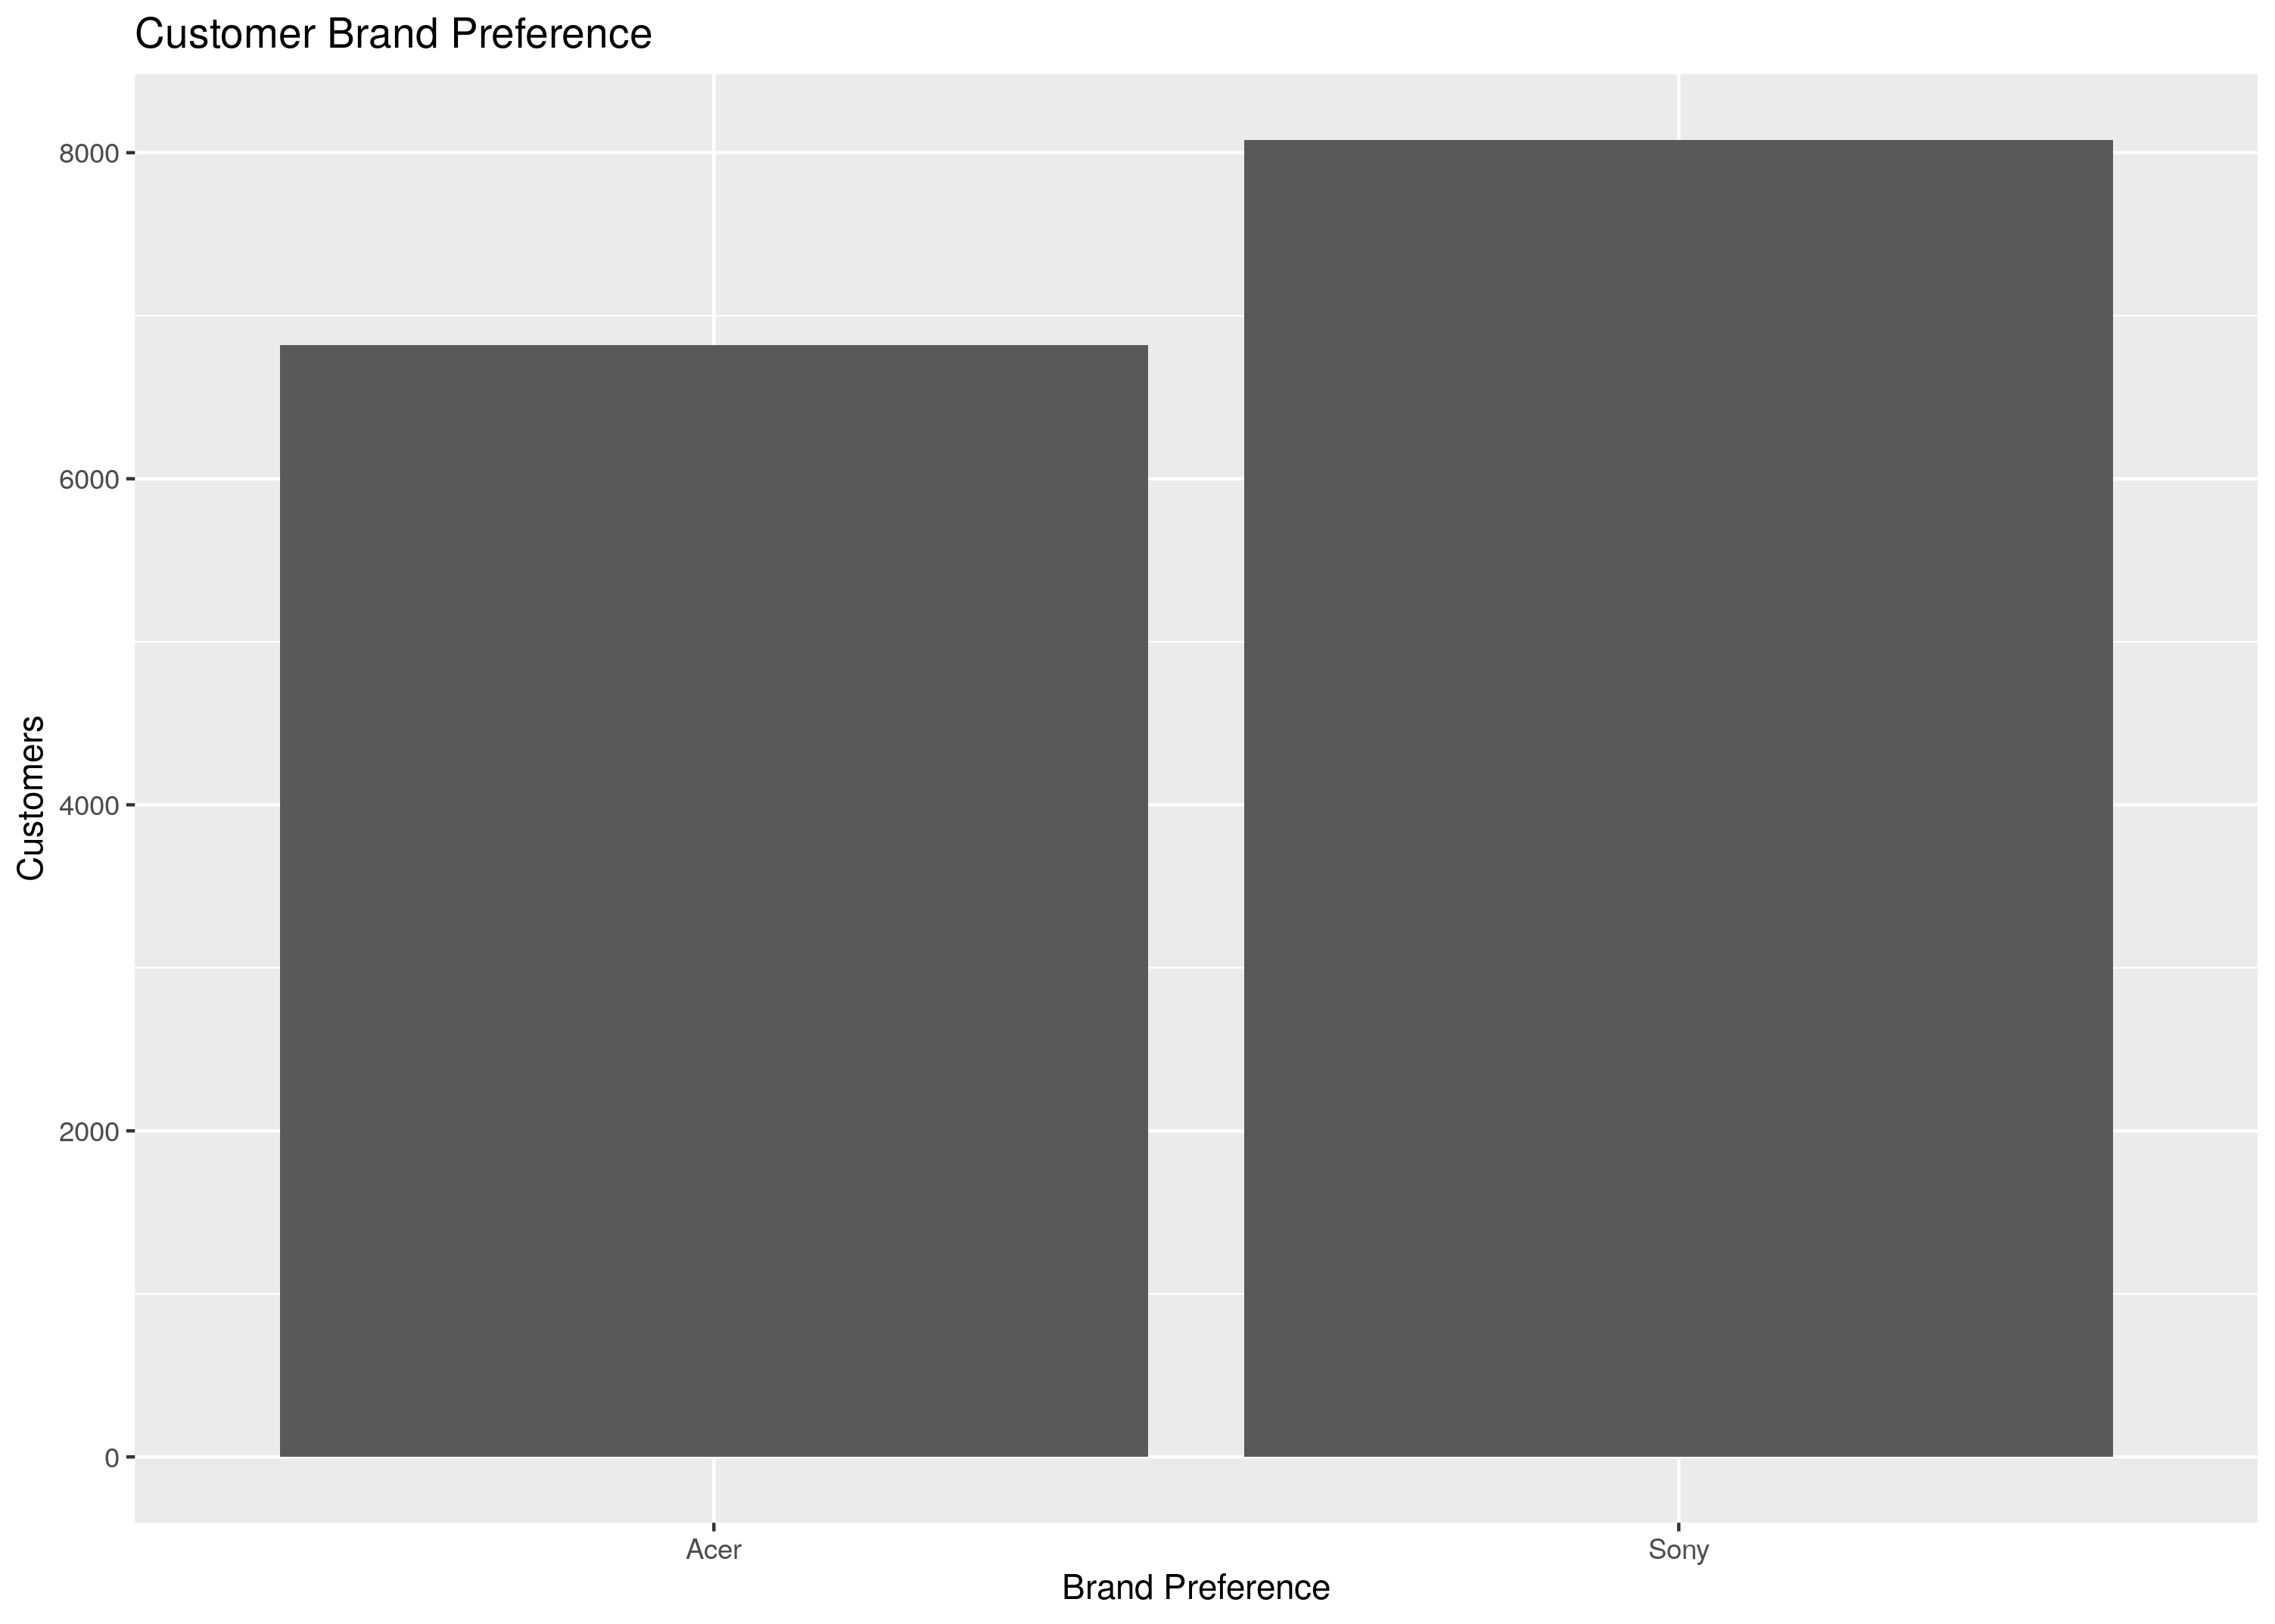
\includegraphics[width=\textwidth,height=\textheight,keepaspectratio]{brand_preference_plain.png}
    \par
}
\bigskip

These are results of the brand preference question after we added in our predictions. We can wee that Sony
is clearly the more preferred brand.

\bigskip
{
    \centering
    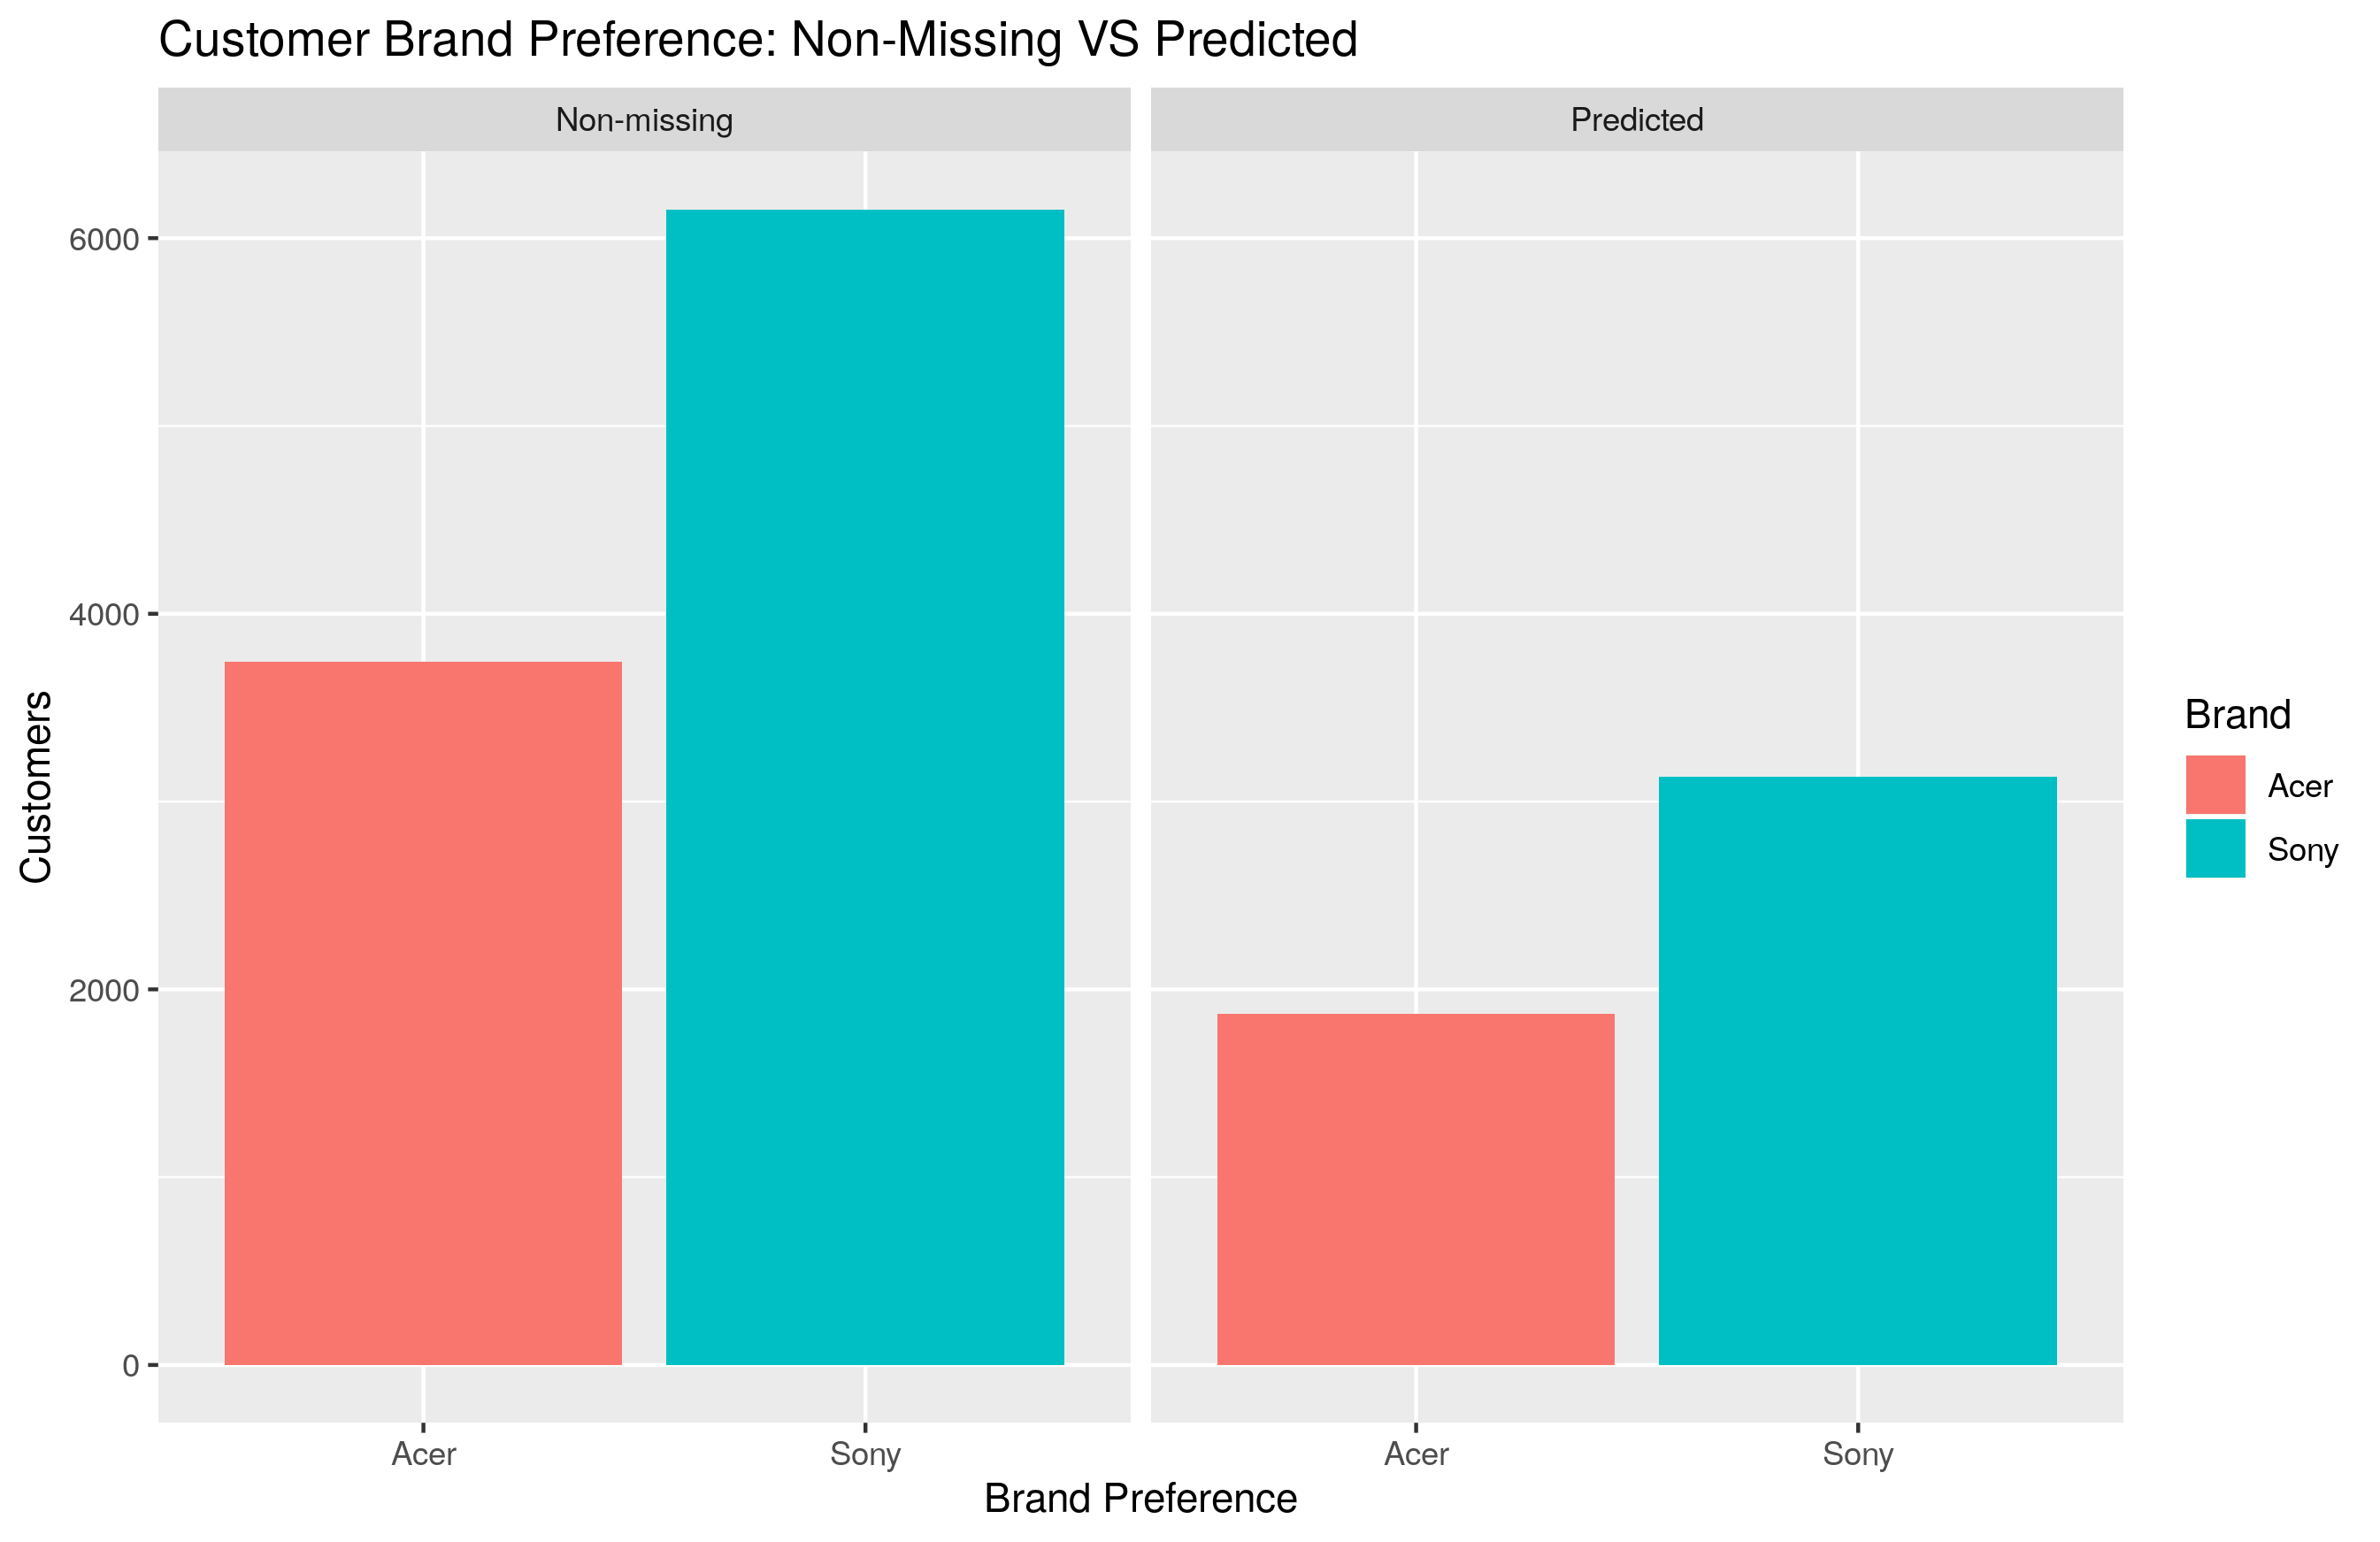
\includegraphics[width=\textwidth,height=\textheight,keepaspectratio]{brand_preference_marked.png}
    \par
}
\bigskip

If we separate from the non-missing answers and the predicted answers, we see
that there were quite a lot of predicted values, but that the brand preference distribution
is the same for both. We can see this even more clearly in a percentage plot.

\bigskip
{
    \centering
    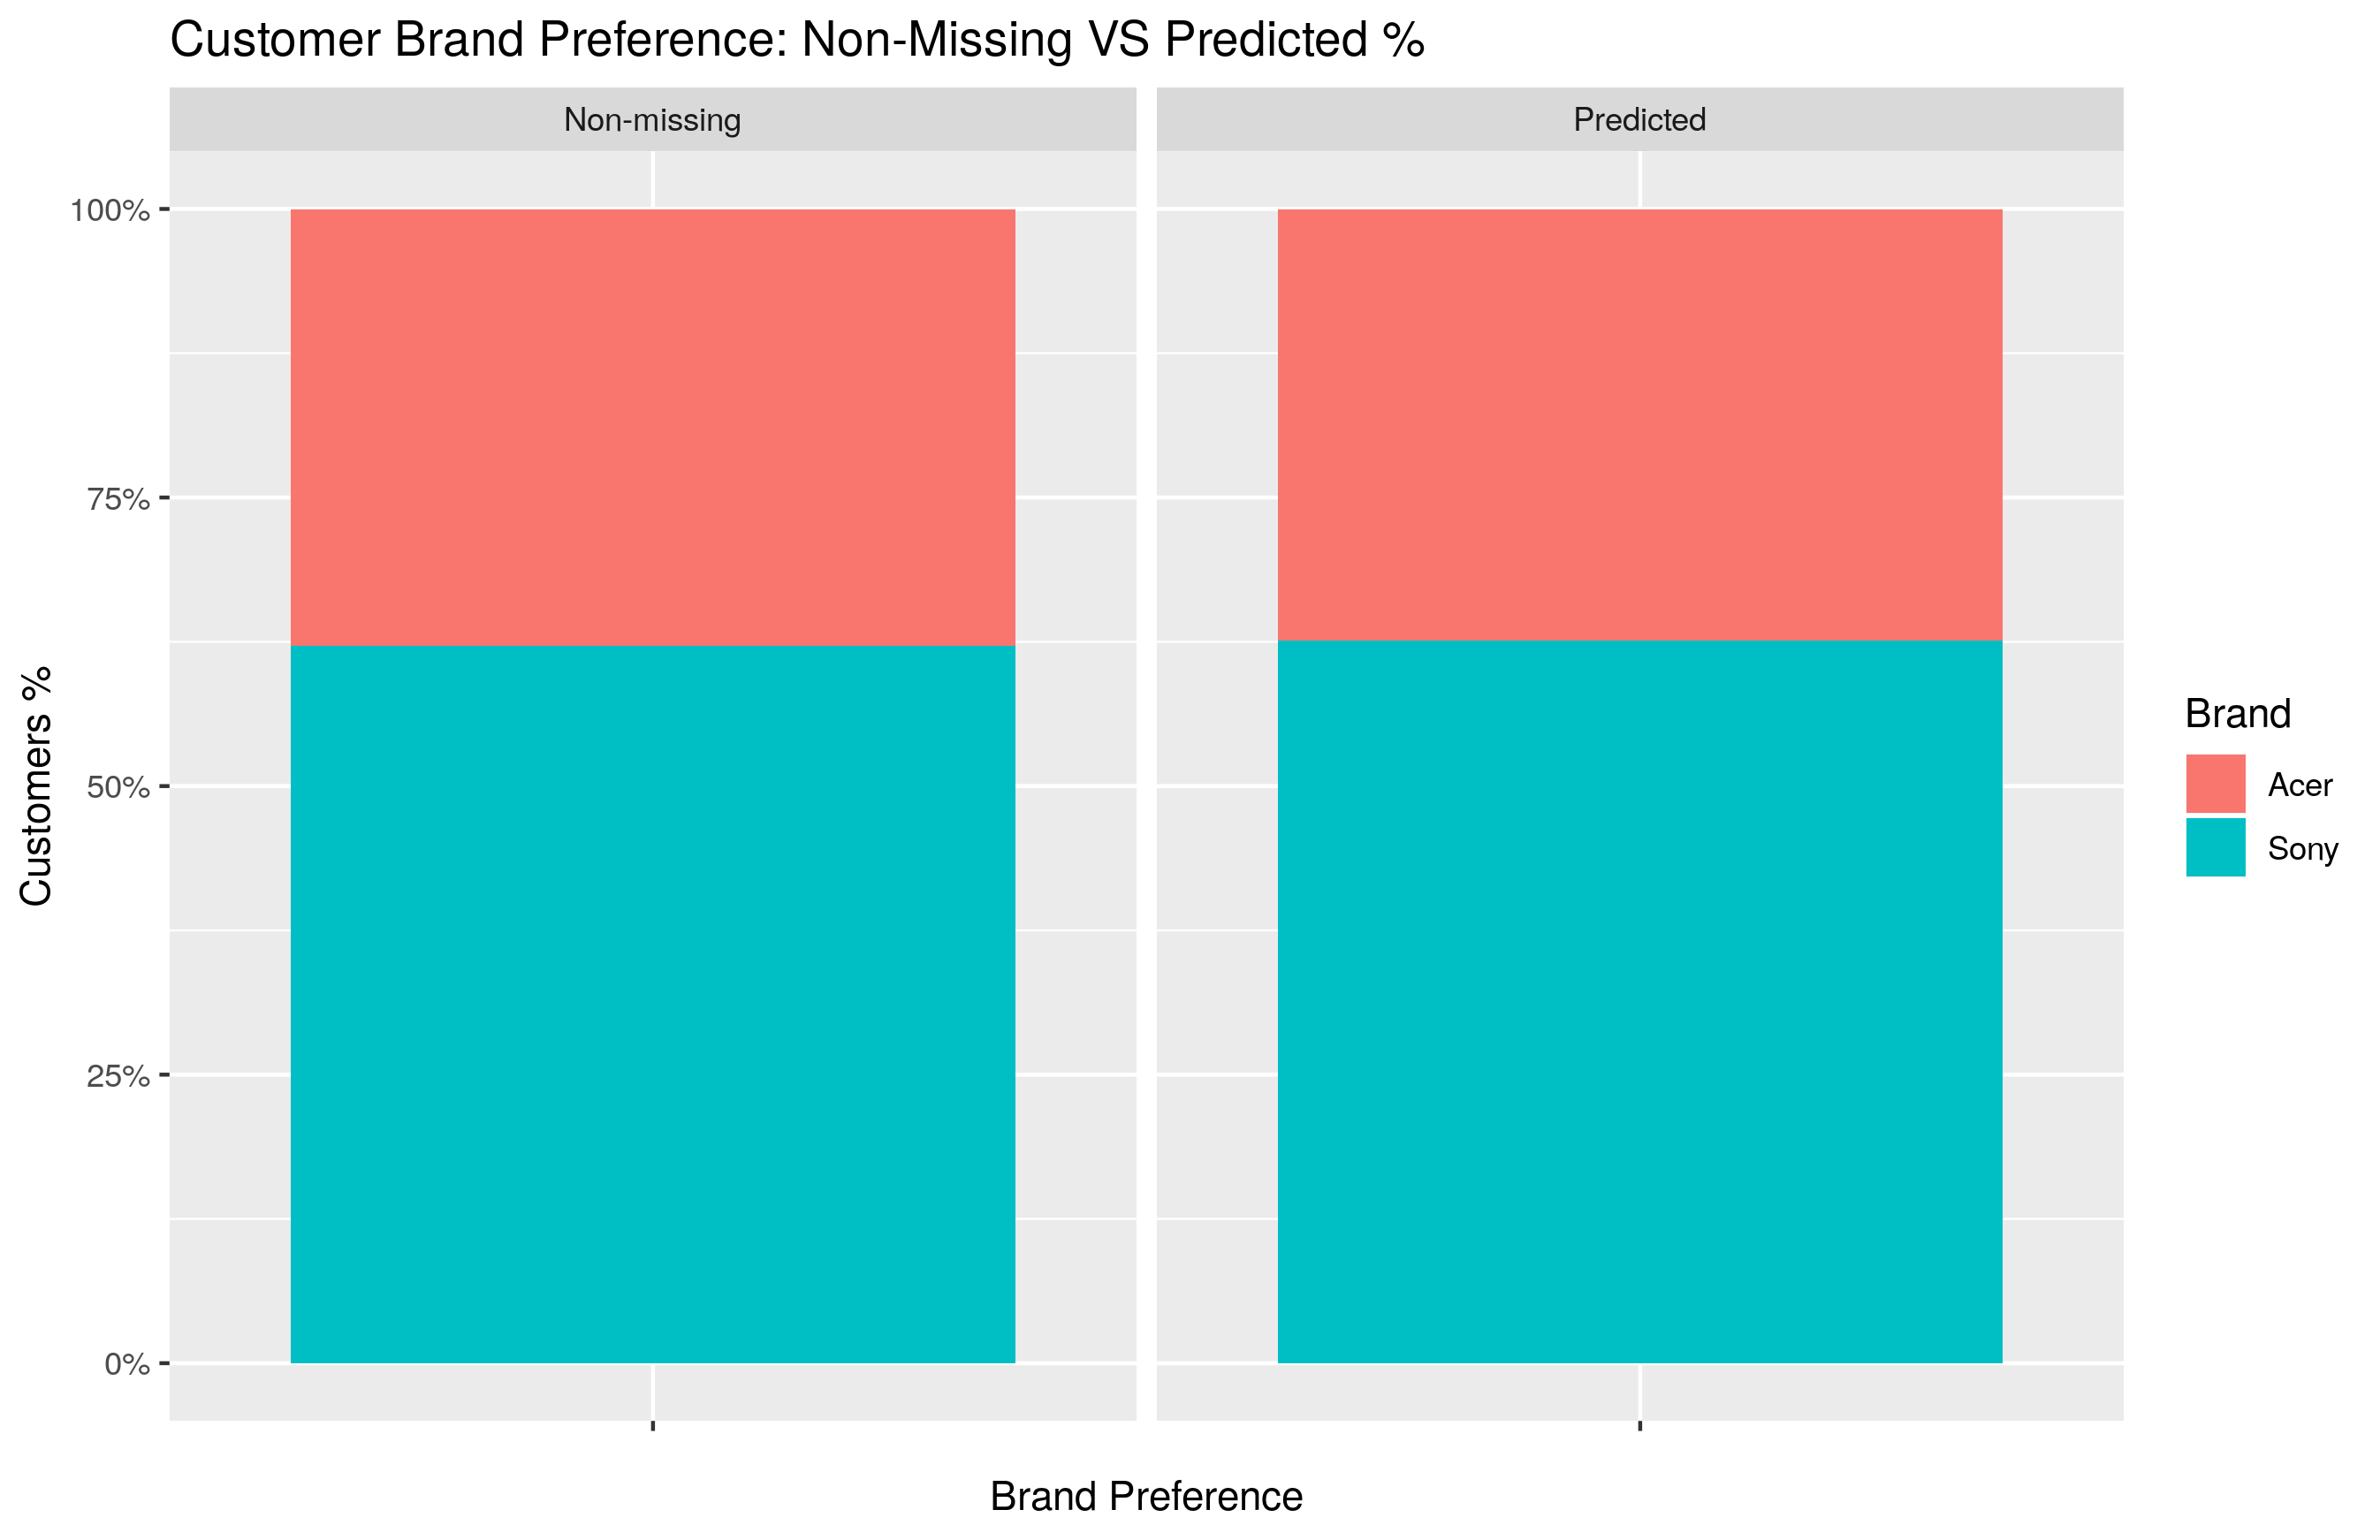
\includegraphics[width=\textwidth,height=\textheight,keepaspectratio]{brand_preference_marked_percentages.png}
    \par
}
\bigskip

If our model is correct (and it is very accurate) this suggests that the missing brand preference values
do not bias our estimate of the brand preference distribution, so in this sense adding in the missing
values does not give any value. On the other hand our model is very accurate and in the future
the answers might not be missing at random. If this is the case, we now have proven that we can make
an accurate model that can correct this bias.

\section{Chosen Model and Its' Performance}

The model used for the predictions is a C5.0 classification tree. From the the graphs below we can see that
on all the important metrics this model performs really well with the train set accuracy being 93.5 \% and
with test set 92.3 \%. This shows that the model is accurate and at the same time
the risk of overfitting is low with the
test and train metrics being so close to each other. This goes for all the other performance metrics as well.

\bigskip
{
    \centering
    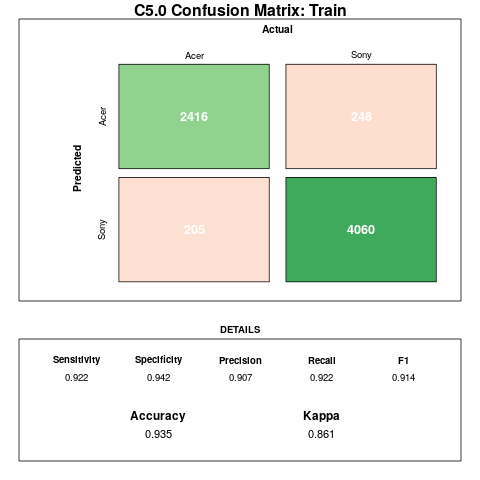
\includegraphics[width=\textwidth,height=\textheight,keepaspectratio]{cm_c5_train.png}
    \par
}
\bigskip

\bigskip
{
    \centering
    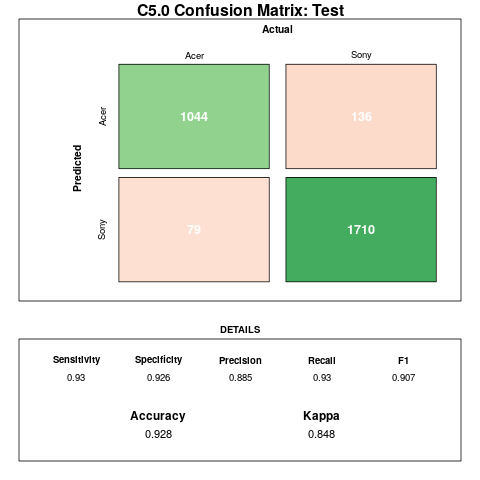
\includegraphics[width=\textwidth,height=\textheight,keepaspectratio]{cm_c5.png}
    \par
}
\bigskip

As the C5.0 decision tree is too complex to understandably visualize. We can instead look at the
relative model feature importances:

\bigskip
{
    \centering
    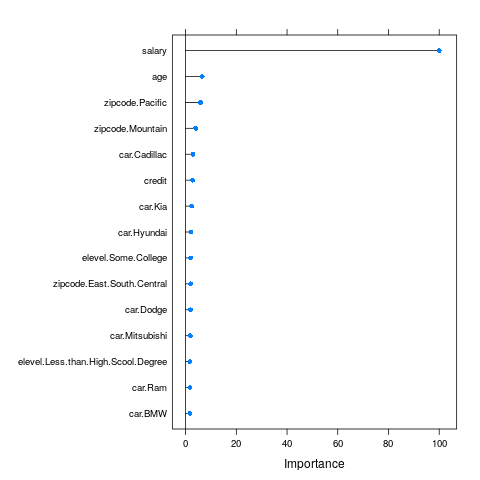
\includegraphics[width=\textwidth,height=\textheight,keepaspectratio]{c5_full_feature_importance.png}
    \par
}
\bigskip

We can see that by far the most import variable is the salary of the customer. If we plot the distribution
of salary with the brand preference, we can see that there are clear differences in brand preference, but that these
are quite complex and nonlinear and would have not been easily captured with a linear model. Tree
type models catch these kind of complex relationships much more easily.

\bigskip
{
    \centering
    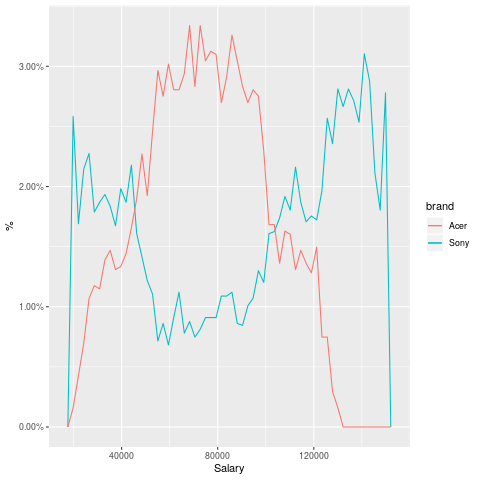
\includegraphics[width=\textwidth,height=\textheight,keepaspectratio]{brand_salary_distribution.png}
    \par
}
\bigskip


\section{Model Comparison and Performance}

In total three different model types were tried: C5.0, Random Forest (RF) and Extreme Gradient Boosting (EGB).
All of these model are tree based models and all performed excellently. This made choosing the right model
quite problematic.

From the cross validation boxplots we can see that all models perform very well in all metrics and that
the results have a tight spread. This suggests that the models have good performance would probably
generalize well to previously unknown data as well.

\bigskip
{
    \centering
    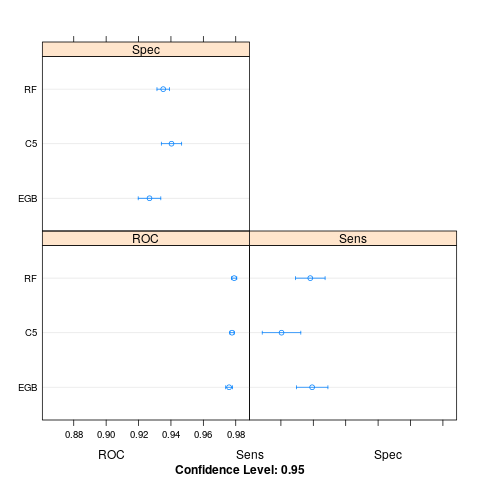
\includegraphics[width=\textwidth,height=\textheight,keepaspectratio]{dotplot_comparison.png}
    \par
}
\bigskip

The small differences between the models can best be seen in the ROC-curve calculated with test data:

\bigskip
{
    \centering
    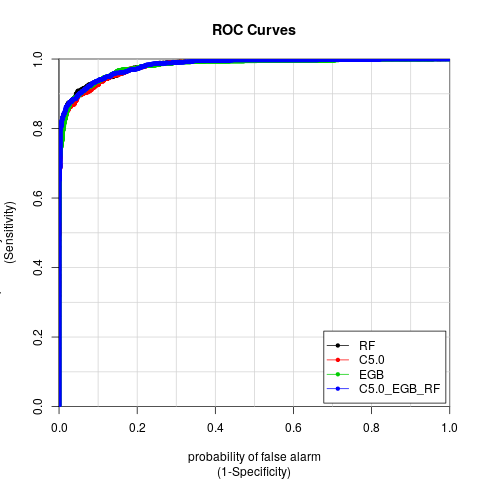
\includegraphics[width=\textwidth,height=\textheight,keepaspectratio]{AUC_comparison.png}
    \par
}
\bigskip

The models are almost indistinguishable, with our chosen C5.0 model maybe somewhat getting a head around
the optimal (Youden Index) point closest to the left upper corner of the graph.

If we look at the results of the other two models more closely, we see that the Random Forest
model has the smallest difference between the metrics from train and test datasets. This
would suggest that this model is the most generalizable of the models tested. It did not
as well as the C5.0 with AUC-measure (previous boxplot) and sensitivity, but beat it on
specificity. The confidence interval of the cross validated metrics were overlapping though
so we can't say with high confidence that C5.0 is strictly better.

\bigskip
{
    \centering
    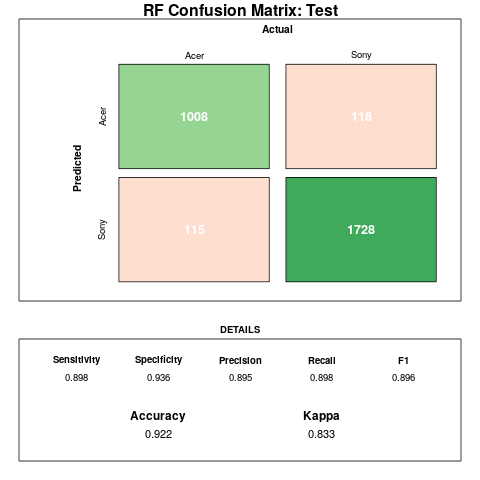
\includegraphics[width=\textwidth,height=\textheight,keepaspectratio]{cm_rf.png}
    \par
}
\bigskip

\bigskip
{
    \centering
    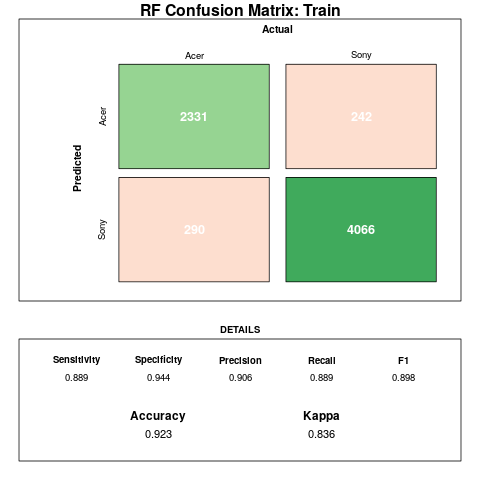
\includegraphics[width=\textwidth,height=\textheight,keepaspectratio]{cm_rf_train.png}
    \par
}
\bigskip

Extreme Gradient Boosting had a metric score difference between train and test datasets, which
was comparable to C5.0 model. It also performed less well than C5.0 on AUC-measure and specificity,
but had the best sensitivity of all the models. All in all also a very good model, but slightly
worse than C5.0 and Random Forest.

\bigskip
{
    \centering
    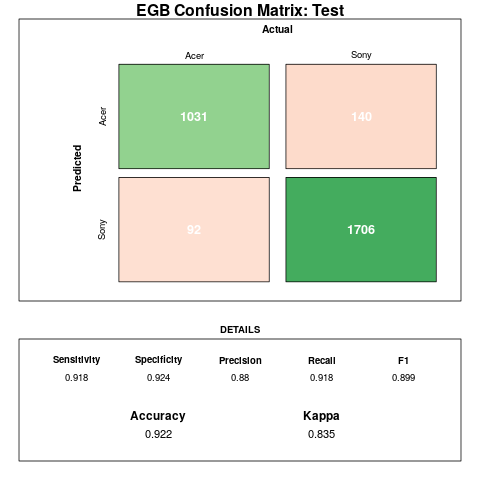
\includegraphics[width=\textwidth,height=\textheight,keepaspectratio]{cm_egb.png}
    \par
}
\bigskip

\bigskip
{
    \centering
    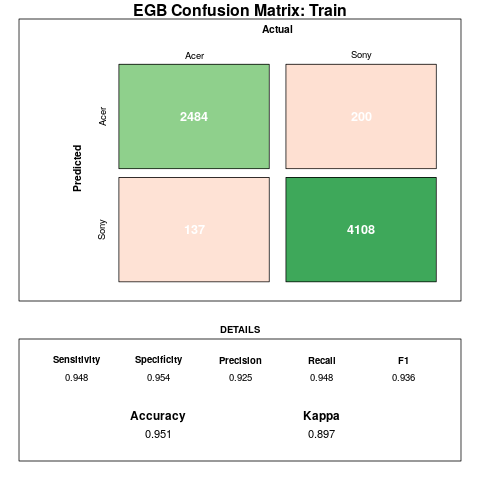
\includegraphics[width=\textwidth,height=\textheight,keepaspectratio]{cm_egb_train.png}
    \par
}
\bigskip

\section{Ensemble Models?}

When looking at the cross validation model AUC-scores we see that the
correlation between these scores is very low between the models
(AUC scores don't line up neatly on the diagonal).

\bigskip
{
    \centering
    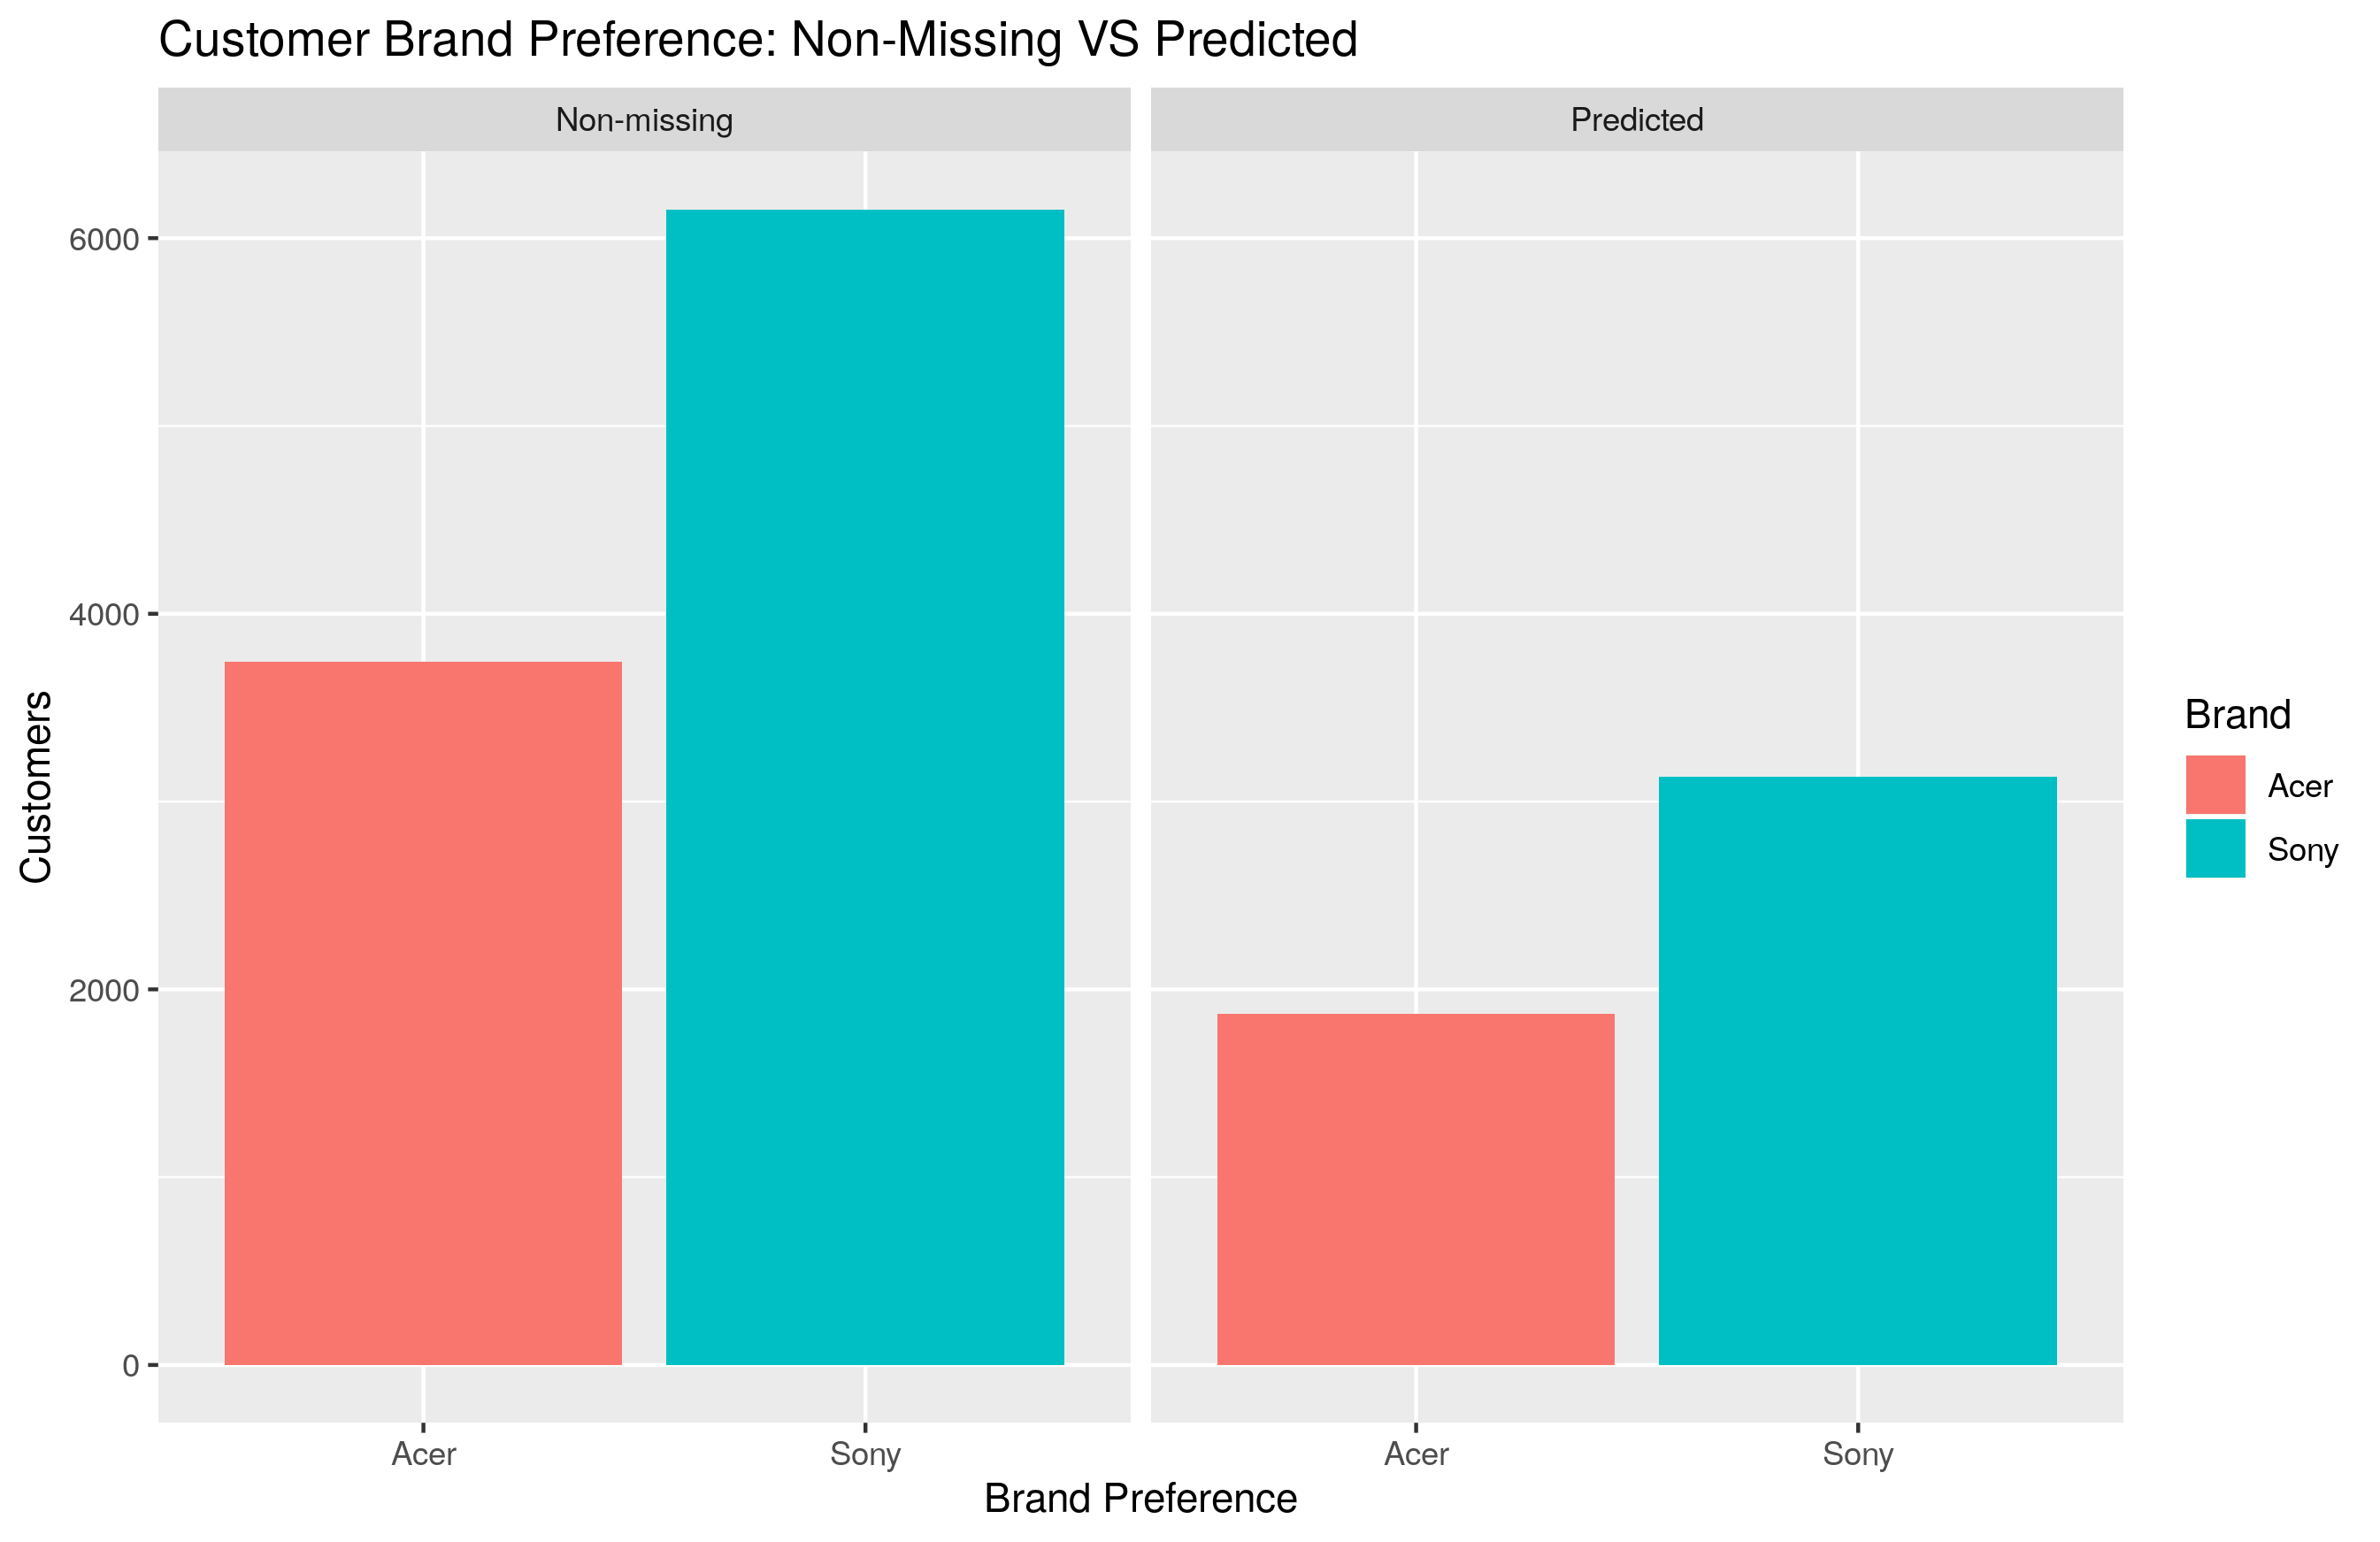
\includegraphics[width=\textwidth,height=\textheight,keepaspectratio]{model_prediction_correlations.png}
    \par
}
\bigskip

This means that the model seem to be making different kinds of mistakes.
We could try to exploit this by building an ensemble model our individual model results.
This was tried, with the best model being a combination of C5.0 and
Random Forest. This model actually had slightly better scores on all metrics
than individual models, but the improvement was very small and at the same
time the model showed signs of overfitting with it having the biggest difference
in performance between train and test set. Because the increase in performance so small
it was deemed unwise to increase the complexity of the model by using an ensemble method.
With the bigger difference between the train and test set this complex model was showing
signs of overfit although it still performed better than other models with the test set.

\end{document}
